% GRL paper template for the Geophysics programs of the University of
% Liverpool. This is part of the submission for the joint Master's program
% dissertation.


%%%%%%%%%%%%%%%%%%%%%%%%%%%%%%%%%%%%%%%%%%%%%%%%%%%%%%%%%%%%%%%%%%%%%%%%%%%%%%%
% Fill these in and they will be set throughout the document
\newcommand{\Name}{%
  Yoür Name
}  % Note that you can use any Unicode character
\newcommand{\Title}{%
  Title of the paper that is really long and will take up multiple lines on the page
}
\newcommand{\Affiliation}{%
  Department of Earth, Ocean, and Ecological Sciences, University of Liverpool, UK
}
%%%%%%%%%%%%%%%%%%%%%%%%%%%%%%%%%%%%%%%%%%%%%%%%%%%%%%%%%%%%%%%%%%%%%%%%%%%%%%%

\documentclass[9pt,twocolumn]{paper}
% Full Unicode support for non-ASCII characters
\usepackage[utf8]{inputenc}
% Typographical rules for English
\usepackage[english]{babel}
% Handling figures in PNG, JPG, PDF, etc
\usepackage{graphicx}
% Better and more extensive maths
\usepackage{amsmath}
% Set the borders of the page
\usepackage[a4paper,left=1.5cm,right=1.5cm,top=2.5cm,bottom=2cm]{geometry}
% Include links and metadata in PDFs
\usepackage[colorlinks=true]{hyperref}
% Nice styling for headers and footers
\usepackage{fancyhdr}
% Formatting the bibliography
\usepackage[round]{natbib}
\usepackage{natbibspacing}
% To make the title a single column
\usepackage{multicol}
% To insert dummy text into this template. Can be removed.
\usepackage{lipsum}

% Set the spacing between columns
\setlength{\columnsep}{0.75cm}

% Setup metadata for the PDF and link colour
\hypersetup{
    pdftitle={\Title},
    pdfauthor={\Name},
    linkcolor=black,
    citecolor=black,
    filecolor=black,
    urlcolor=blue
}

% Set fancy headers
\usepackage{fancyhdr}
\pagestyle{fancy}
\fancyhf{}
\lhead{}
\chead{}
\rhead{\fontsize{9pt}{0}\selectfont \thepage}
\cfoot{}
\renewcommand{\headrulewidth}{0pt}


\begin{document}

% Insert the title, name, and affiliation. All of this is set at the very top
% of the file. DON'T CHANGE THINGS HERE.
\twocolumn[
  \begin{@twocolumnfalse}
    \noindent \textbf{\large \Title{}}
  \end{@twocolumnfalse}
  \vspace{0.7cm}
]
\noindent {\large \Name{}}
\\[0.2cm]
\noindent {\small \Affiliation{}}
\vspace{0.5cm}

%%%%%%%%%%%%%%%%%%%%%%%%%%%%%%%%%%%%%%%%%%%%%%%%%%%%%%%%%%%%%%%%%%%%%%%%%%%%%%%
\noindent
\textbf{Abstract.}
Insert abstract here. Don't include any blank lines.
\lipsum[1]

%%%%%%%%%%%%%%%%%%%%%%%%%%%%%%%%%%%%%%%%%%%%%%%%%%%%%%%%%%%%%%%%%%%%%%%%%%%%%%%
\section{Introduction}

Make some citations: \cite{Parker1973} or \citep{Parker1973}.
The following is just filler text.
\lipsum[1-4]


%%%%%%%%%%%%%%%%%%%%%%%%%%%%%%%%%%%%%%%%%%%%%%%%%%%%%%%%%%%%%%%%%%%%%%%%%%%%%%%
\section{Methods}

Examples of equations in eq.~\ref{eq:linear_least_squares} and figures in
fig.~\ref{fig:example}.

\begin{equation}
  \mathbf{\hat{p}} =
    \left(\mathbf{A}^T\mathbf{A}\right)^{-1}
    \mathbf{A}^T\mathbf{d^o}
  % Label used to reference the equation in the text.
  \label{eq:linear_least_squares}
\end{equation}

\begin{figure}[!htb]
  % Width should be \columnwidth for a single column
  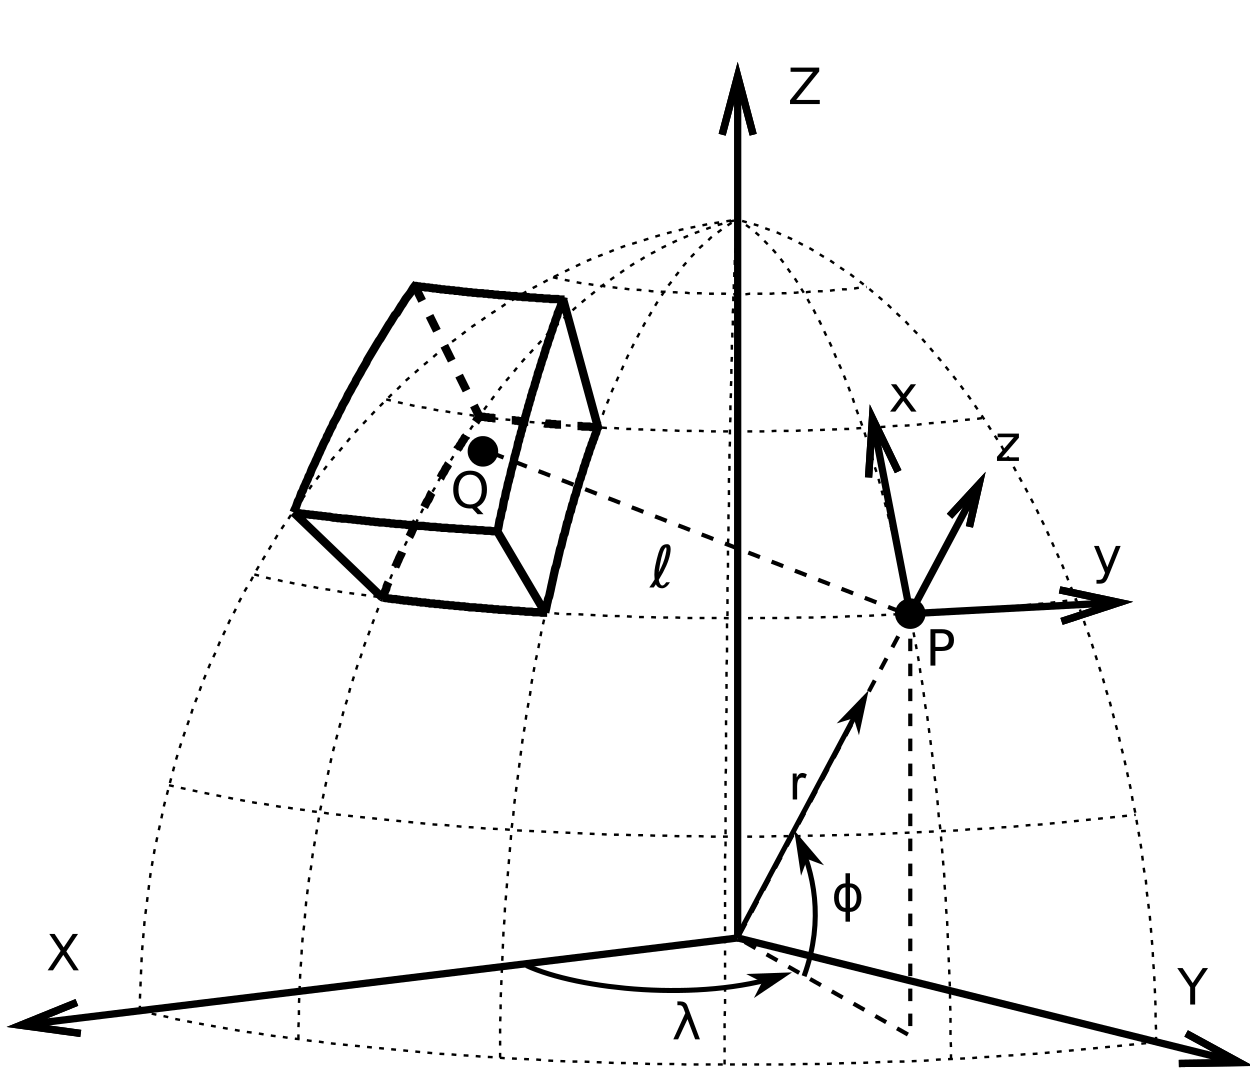
\includegraphics[width=\columnwidth]{figures/tesseroid-coord-sys.png}
  \caption{
    This is the figure caption. Notice that the figure number is inserted into
    the text automatically. After \citet{uieda2015}.
  }
  % Label used to reference the figure in the text.
  \label{fig:example}
\end{figure}

\lipsum[2-4]


%%%%%%%%%%%%%%%%%%%%%%%%%%%%%%%%%%%%%%%%%%%%%%%%%%%%%%%%%%%%%%%%%%%%%%%%%%%%%%%
\section{Results}

Example of a 2 column figure (avoid these if you can):
fig.~\ref{fig:example_fullpage}.
\lipsum[4]

\begin{figure*}[!htb]
  % Width should be \textwidth for full page figures
  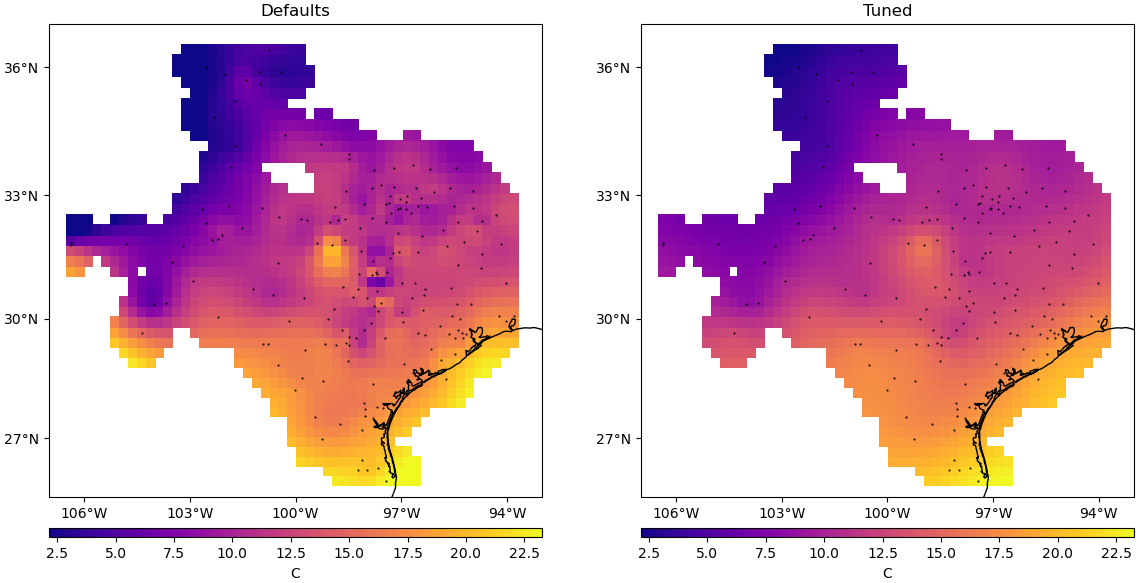
\includegraphics[width=\textwidth]{figures/example-spline-interpolation.png}
  \caption{
    Another figure with full page width. Avoid these if you can since they are
    tricky to place in the text.
  }
  % Label used to reference the figure in the text.
  \label{fig:example_fullpage}
\end{figure*}

\lipsum[5-8]


%%%%%%%%%%%%%%%%%%%%%%%%%%%%%%%%%%%%%%%%%%%%%%%%%%%%%%%%%%%%%%%%%%%%%%%%%%%%%%%
\section{Discussion}

\lipsum[4-8]


%%%%%%%%%%%%%%%%%%%%%%%%%%%%%%%%%%%%%%%%%%%%%%%%%%%%%%%%%%%%%%%%%%%%%%%%%%%%%%%
\section{Conclusions}

\lipsum[8]



%%%%%%%%%%%%%%%%%%%%%%%%%%%%%%%%%%%%%%%%%%%%%%%%%%%%%%%%%%%%%%%%%%%%%%%%%%%%%%%
\vspace{0.5cm}
\noindent
{\small
  \textbf{Acknowledgments.}
  Add your acknowledgements here. Don't put any blank lines.
}


%%%%%%%%%%%%%%%%%%%%%%%%%%%%%%%%%%%%%%%%%%%%%%%%%%%%%%%%%%%%%%%%%%%%%%%%%%%%%%%
% Use the American Geophysical Union citation style
\bibliographystyle{agu}
% The References section is automatically populated from the cited entries of
% the references.bib file
\bibliography{references}

\vspace{0.3cm}
\noindent
{\footnotesize
  Mailing address: School of Environmental Sciences, University, of
  Liverpool, Jane Herdman Building, Liverpool L69 3GP, United Kingdom
}

\end{document}

